% Options for packages loaded elsewhere
\PassOptionsToPackage{unicode}{hyperref}
\PassOptionsToPackage{hyphens}{url}
%
\documentclass[
]{article}
\usepackage{amsmath,amssymb}
\usepackage{lmodern}
\usepackage{ifxetex,ifluatex}
\ifnum 0\ifxetex 1\fi\ifluatex 1\fi=0 % if pdftex
  \usepackage[T1]{fontenc}
  \usepackage[utf8]{inputenc}
  \usepackage{textcomp} % provide euro and other symbols
\else % if luatex or xetex
  \usepackage{unicode-math}
  \defaultfontfeatures{Scale=MatchLowercase}
  \defaultfontfeatures[\rmfamily]{Ligatures=TeX,Scale=1}
\fi
% Use upquote if available, for straight quotes in verbatim environments
\IfFileExists{upquote.sty}{\usepackage{upquote}}{}
\IfFileExists{microtype.sty}{% use microtype if available
  \usepackage[]{microtype}
  \UseMicrotypeSet[protrusion]{basicmath} % disable protrusion for tt fonts
}{}
\makeatletter
\@ifundefined{KOMAClassName}{% if non-KOMA class
  \IfFileExists{parskip.sty}{%
    \usepackage{parskip}
  }{% else
    \setlength{\parindent}{0pt}
    \setlength{\parskip}{6pt plus 2pt minus 1pt}}
}{% if KOMA class
  \KOMAoptions{parskip=half}}
\makeatother
\usepackage{xcolor}
\IfFileExists{xurl.sty}{\usepackage{xurl}}{} % add URL line breaks if available
\IfFileExists{bookmark.sty}{\usepackage{bookmark}}{\usepackage{hyperref}}
\hypersetup{
  hidelinks,
  pdfcreator={LaTeX via pandoc}}
\urlstyle{same} % disable monospaced font for URLs
\usepackage[margin=1in]{geometry}
\usepackage{color}
\usepackage{fancyvrb}
\newcommand{\VerbBar}{|}
\newcommand{\VERB}{\Verb[commandchars=\\\{\}]}
\DefineVerbatimEnvironment{Highlighting}{Verbatim}{commandchars=\\\{\}}
% Add ',fontsize=\small' for more characters per line
\usepackage{framed}
\definecolor{shadecolor}{RGB}{35,38,41}
\newenvironment{Shaded}{\begin{snugshade}}{\end{snugshade}}
\newcommand{\AlertTok}[1]{\textcolor[rgb]{0.58,0.85,0.30}{\textbf{\colorbox[rgb]{0.30,0.12,0.14}{#1}}}}
\newcommand{\AnnotationTok}[1]{\textcolor[rgb]{0.25,0.50,0.35}{#1}}
\newcommand{\AttributeTok}[1]{\textcolor[rgb]{0.16,0.50,0.73}{#1}}
\newcommand{\BaseNTok}[1]{\textcolor[rgb]{0.96,0.45,0.00}{#1}}
\newcommand{\BuiltInTok}[1]{\textcolor[rgb]{0.50,0.55,0.55}{#1}}
\newcommand{\CharTok}[1]{\textcolor[rgb]{0.24,0.68,0.91}{#1}}
\newcommand{\CommentTok}[1]{\textcolor[rgb]{0.48,0.49,0.49}{#1}}
\newcommand{\CommentVarTok}[1]{\textcolor[rgb]{0.50,0.55,0.55}{#1}}
\newcommand{\ConstantTok}[1]{\textcolor[rgb]{0.15,0.68,0.68}{\textbf{#1}}}
\newcommand{\ControlFlowTok}[1]{\textcolor[rgb]{0.99,0.74,0.29}{\textbf{#1}}}
\newcommand{\DataTypeTok}[1]{\textcolor[rgb]{0.16,0.50,0.73}{#1}}
\newcommand{\DecValTok}[1]{\textcolor[rgb]{0.96,0.45,0.00}{#1}}
\newcommand{\DocumentationTok}[1]{\textcolor[rgb]{0.64,0.20,0.25}{#1}}
\newcommand{\ErrorTok}[1]{\textcolor[rgb]{0.85,0.27,0.33}{\underline{#1}}}
\newcommand{\ExtensionTok}[1]{\textcolor[rgb]{0.00,0.60,1.00}{\textbf{#1}}}
\newcommand{\FloatTok}[1]{\textcolor[rgb]{0.96,0.45,0.00}{#1}}
\newcommand{\FunctionTok}[1]{\textcolor[rgb]{0.56,0.27,0.68}{#1}}
\newcommand{\ImportTok}[1]{\textcolor[rgb]{0.15,0.68,0.38}{#1}}
\newcommand{\InformationTok}[1]{\textcolor[rgb]{0.77,0.36,0.00}{#1}}
\newcommand{\KeywordTok}[1]{\textcolor[rgb]{0.81,0.81,0.76}{\textbf{#1}}}
\newcommand{\NormalTok}[1]{\textcolor[rgb]{0.81,0.81,0.76}{#1}}
\newcommand{\OperatorTok}[1]{\textcolor[rgb]{0.81,0.81,0.76}{#1}}
\newcommand{\OtherTok}[1]{\textcolor[rgb]{0.15,0.68,0.38}{#1}}
\newcommand{\PreprocessorTok}[1]{\textcolor[rgb]{0.15,0.68,0.38}{#1}}
\newcommand{\RegionMarkerTok}[1]{\textcolor[rgb]{0.16,0.50,0.73}{\colorbox[rgb]{0.08,0.19,0.26}{#1}}}
\newcommand{\SpecialCharTok}[1]{\textcolor[rgb]{0.24,0.68,0.91}{#1}}
\newcommand{\SpecialStringTok}[1]{\textcolor[rgb]{0.85,0.27,0.33}{#1}}
\newcommand{\StringTok}[1]{\textcolor[rgb]{0.96,0.31,0.31}{#1}}
\newcommand{\VariableTok}[1]{\textcolor[rgb]{0.15,0.68,0.68}{#1}}
\newcommand{\VerbatimStringTok}[1]{\textcolor[rgb]{0.85,0.27,0.33}{#1}}
\newcommand{\WarningTok}[1]{\textcolor[rgb]{0.85,0.27,0.33}{#1}}
\usepackage{graphicx}
\makeatletter
\def\maxwidth{\ifdim\Gin@nat@width>\linewidth\linewidth\else\Gin@nat@width\fi}
\def\maxheight{\ifdim\Gin@nat@height>\textheight\textheight\else\Gin@nat@height\fi}
\makeatother
% Scale images if necessary, so that they will not overflow the page
% margins by default, and it is still possible to overwrite the defaults
% using explicit options in \includegraphics[width, height, ...]{}
\setkeys{Gin}{width=\maxwidth,height=\maxheight,keepaspectratio}
% Set default figure placement to htbp
\makeatletter
\def\fps@figure{htbp}
\makeatother
\setlength{\emergencystretch}{3em} % prevent overfull lines
\providecommand{\tightlist}{%
  \setlength{\itemsep}{0pt}\setlength{\parskip}{0pt}}
\setcounter{secnumdepth}{5}
\ifluatex
  \usepackage{selnolig}  % disable illegal ligatures
\fi

\title{Expressed Variant Reporting}
\author{Brandon Michael Blobner, Jenny Leopoldina Smith, and Ahmad Al
Khleifat}
\date{2021-04-14}

\begin{document}
\maketitle

{
\setcounter{tocdepth}{3}
\tableofcontents
}
\hypertarget{about-the-test-variant-detection-from-rna-seq}{%
\section{About The Test: Variant Detection from
RNA-seq}\label{about-the-test-variant-detection-from-rna-seq}}

\begin{figure}

{\centering 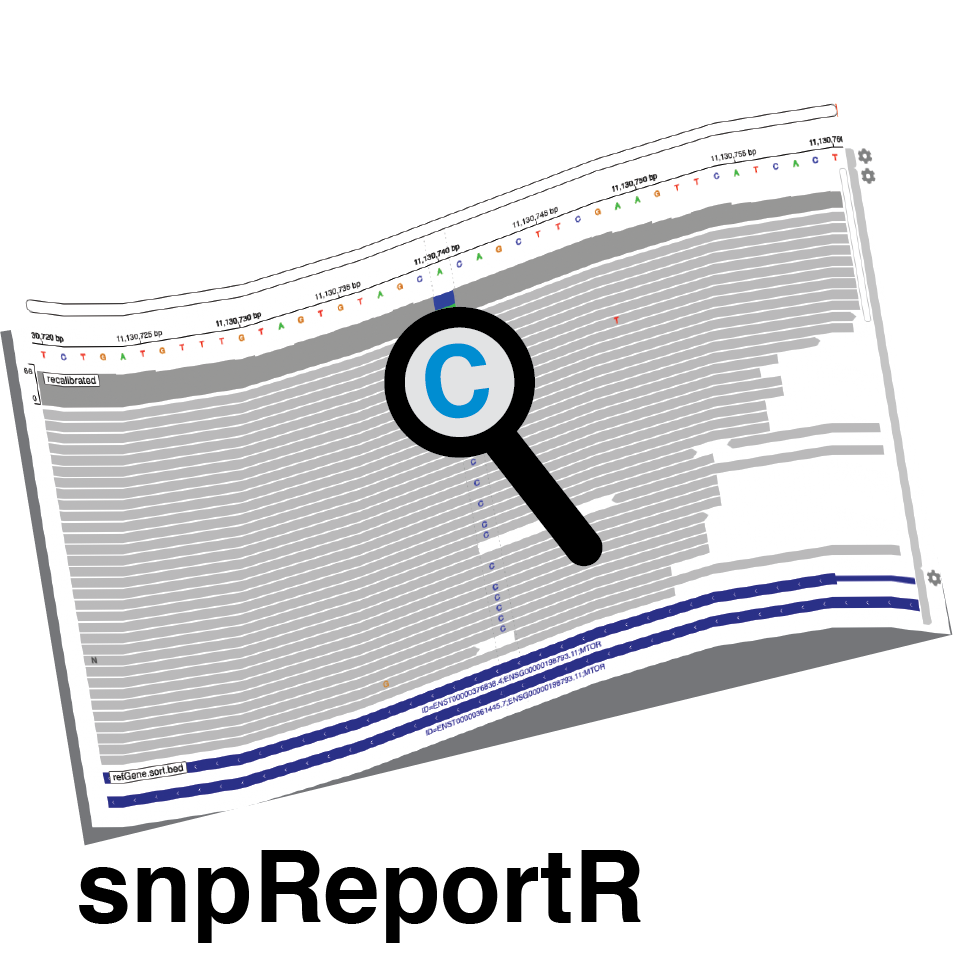
\includegraphics[width=0.25\linewidth]{/Users/jlsmith3/expressed-variant-reporting/logos/snpReporter_logo} 

}

\caption{snpReportR: A Method for RNAseq Variant Detection Reporting}\label{fig:unnamed-chunk-3}
\end{figure}

Patient details:

Information

Value

Name:

Jane Doe

DOB:

01/01/1900

Sex:

F

Sample Type:

RNA

Test ordered by:

Information

Value

Name:

Dr.X

Doctor identification number:

12345

Hospital:

NCI

This document will help you to understand the more important findings
from a gene variant screening. The common definitions of the type of
genetic variants (mutations) are described in the figure and in the
table in section
\texttt{Chromosome\ and\ Gene\ Vizualization\ of\ Mutations}.

While a variant may have been detected, the associations with the
variant are not perfectly causal and their complex interactions between
biology and the environment.

\begin{center}\rule{0.5\linewidth}{0.5pt}\end{center}

\hypertarget{about-the-dataset}{%
\section{About the Dataset}\label{about-the-dataset}}

\begin{figure}

{\centering \includegraphics{/Users/jlsmith3/expressed-variant-reporting/reports/Report_HTML_v2_JSmith_files/figure-latex/unnamed-chunk-9-1} 

}

\caption{Table 1. Column names and Descriptions}\label{fig:unnamed-chunk-9}
\end{figure}

\emph{In addition there are functional annotations for the variants per
transcript from snpEFF. These include:}

\begin{itemize}
\tightlist
\item
  ``Annotation\_Impact''
\item
  ``Feature\_Type''
\item
  ``Transcript\_BioType''
\item
  ``Rank''
\item
  ``HGVS.c''
\item
  ``HGVS.p''
\item
  ``cDNA.pos/cDNA.length''
\item
  ``CDS.pos/CDS.length''
\item
  ``AA.pos/AA.length''
\item
  ``Distance''
\end{itemize}

\emph{The top variants were ranked by the following attributes:}

\begin{itemize}
\tightlist
\item
  FATHMM predicted pathogenicty or splice adjacent
\item
  CHASMplus predicts driver mutations
\item
  genes with larger number of SNVs prioritized
\item
  high or moderate impact on the structure of the gene
\item
  CADD Score/Polyphen Score (not done yet)
\end{itemize}

\emph{Interpretation of attributes}

\begin{itemize}
\tightlist
\item
  ``{[}FATHMM{]} weighted algorithm is capable of adjusting our
  conservation-based predictions to account for the tolerance of related
  sequences to mutations''
  (\url{http://fathmm.biocompute.org.uk/inherited.html})
\item
  ``CHASMplus scores range from 0 to 1, with higher scores meaning more
  likely to be a cancer driver mutation.''
  (\url{https://chasmplus.readthedocs.io/en/latest/})
\item
  ``VEST‐indel scores were assigned to categories of pathogenic (≥0.5)
  or benign (\textless0.5).'' (\url{https://doi.org/10.1002/humu.22911})
\end{itemize}

\begin{center}\includegraphics{/Users/jlsmith3/expressed-variant-reporting/reports/Report_HTML_v2_JSmith_files/figure-latex/unnamed-chunk-11-1} \end{center}

\begin{center}\rule{0.5\linewidth}{0.5pt}\end{center}

\hypertarget{humanmine-annotation-for-further-results}{%
\section{HumanMine Annotation for Further
Results}\label{humanmine-annotation-for-further-results}}

\begin{verbatim}
## [1] "PLK1"  "PDIA6" "FGL1"
\end{verbatim}

\begin{center}\includegraphics{/Users/jlsmith3/expressed-variant-reporting/reports/Report_HTML_v2_JSmith_files/figure-latex/unnamed-chunk-14-1} \end{center}

\begin{figure}

{\centering 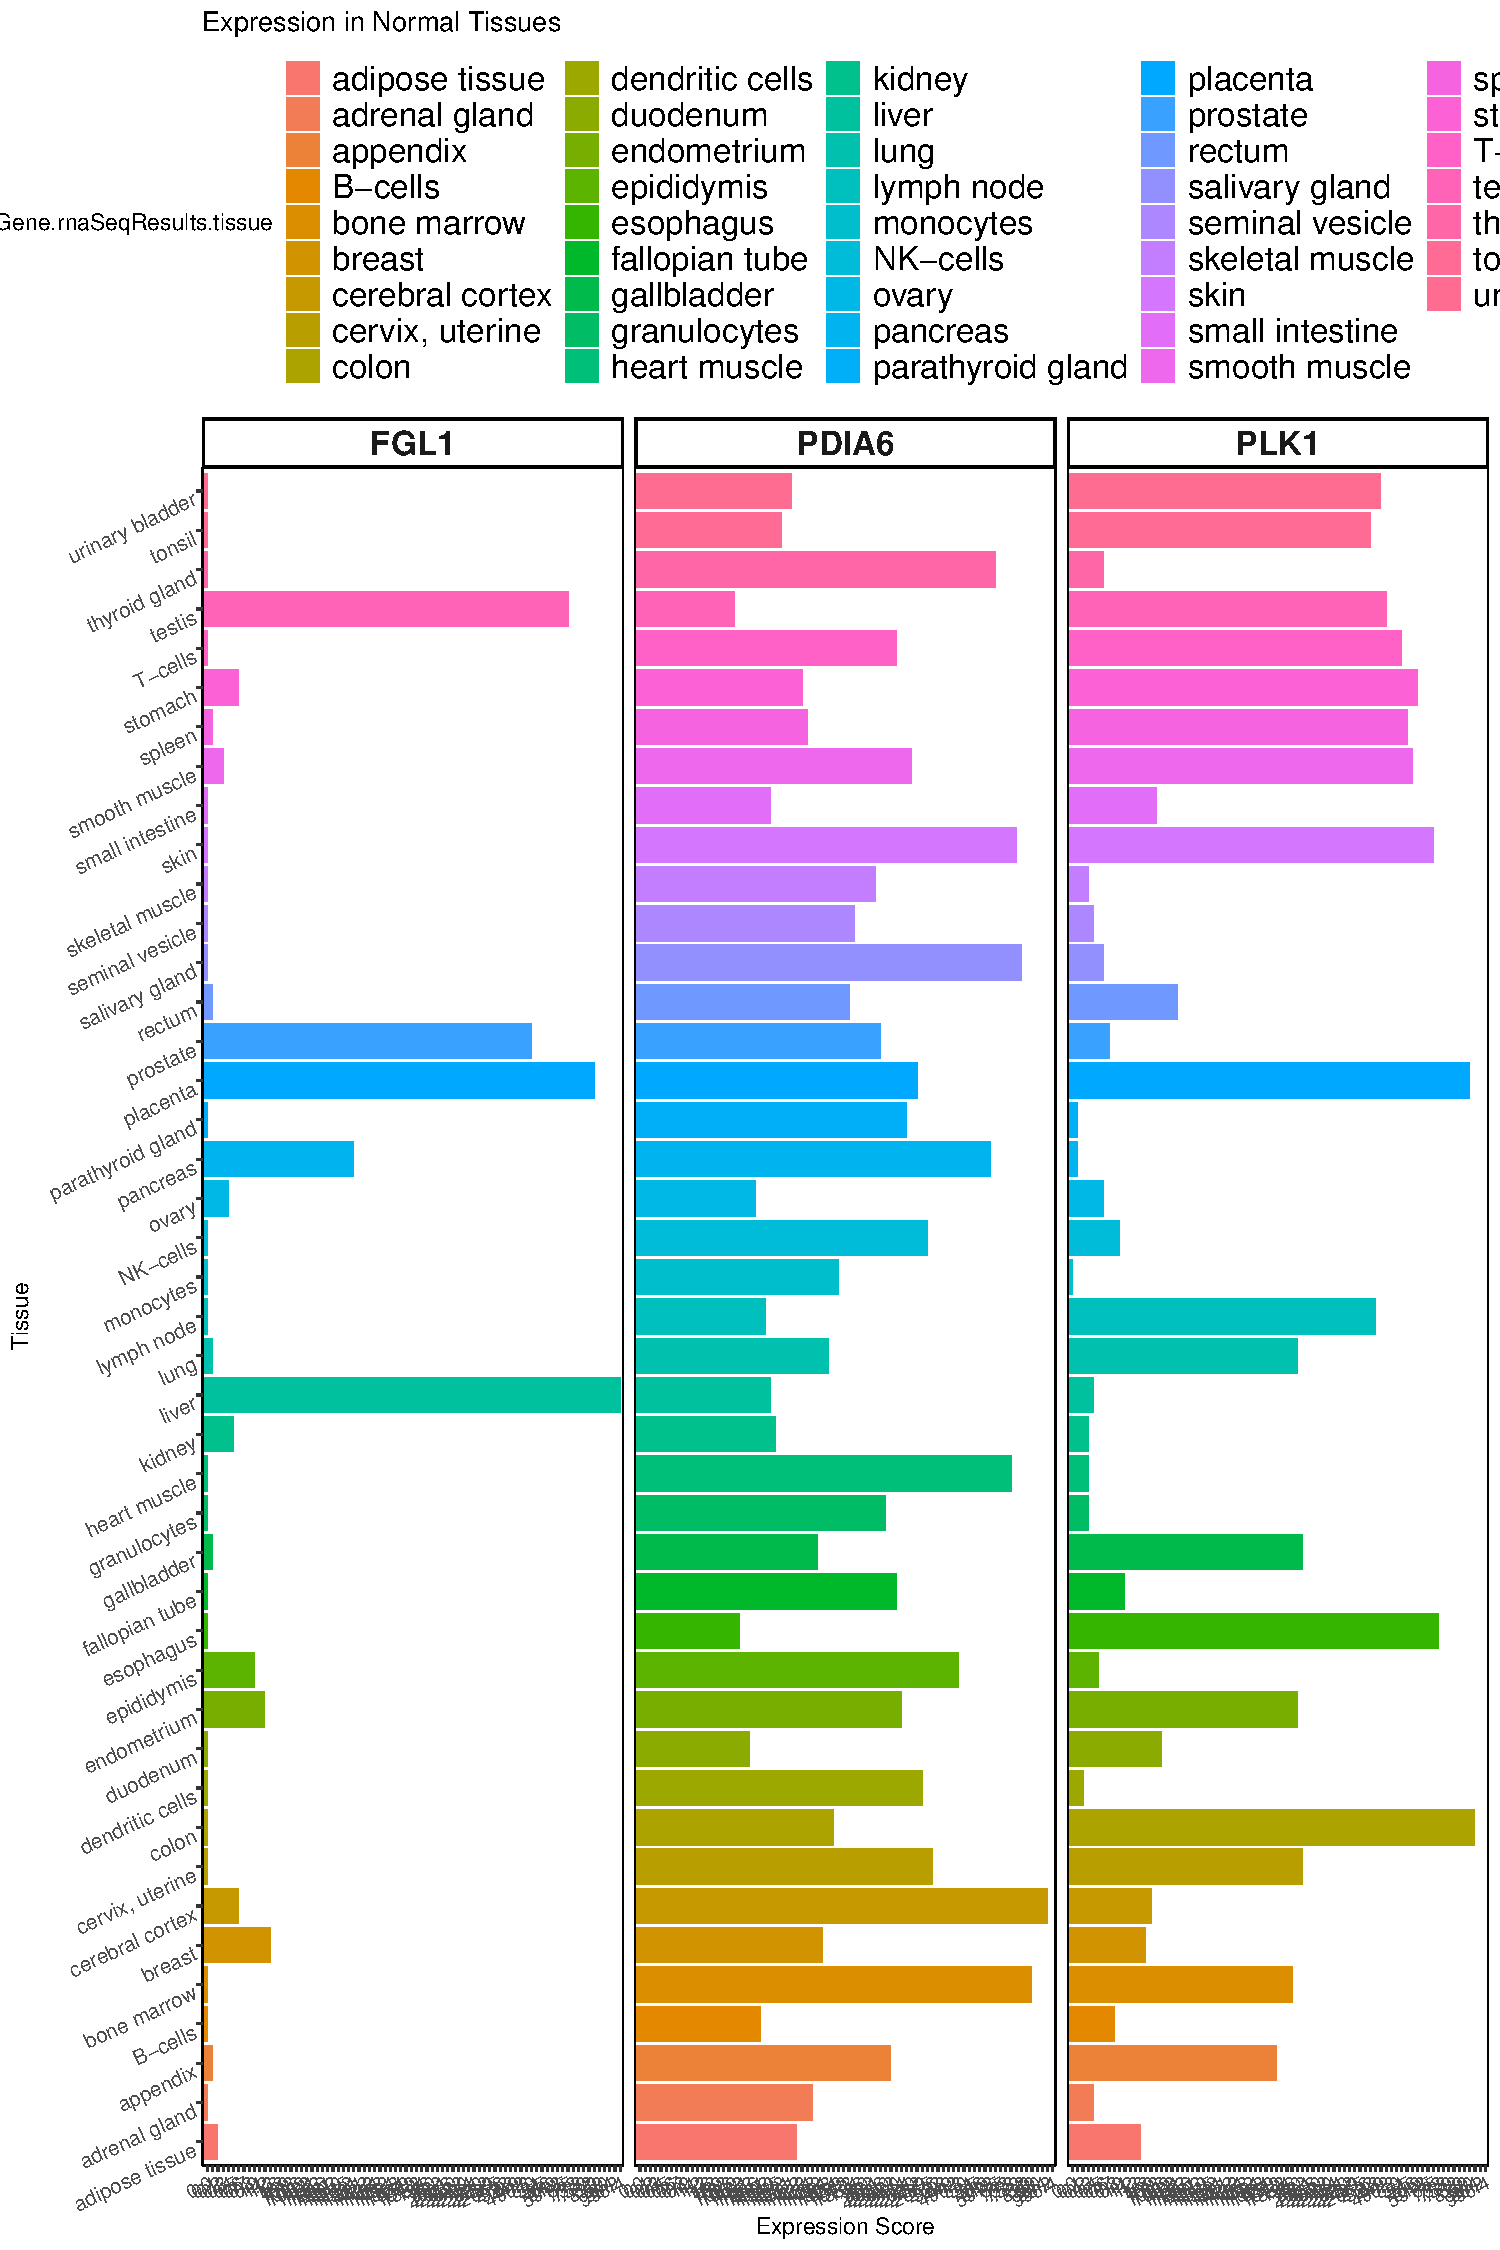
\includegraphics{/Users/jlsmith3/expressed-variant-reporting/reports/Report_HTML_v2_JSmith_files/figure-latex/unnamed-chunk-15-1} 

}

\caption{Expression of Genes with identified variants/SNVs in Normal Tissues.}\label{fig:unnamed-chunk-15}
\end{figure}

\begin{center}\rule{0.5\linewidth}{0.5pt}\end{center}

\hypertarget{results-table}{%
\section{Results Table}\label{results-table}}

Included here are two tables for different gene types. Coding refers to
genes that produce proteins, while non-coding refers to genes which do
get utilized to produce proteins.

\hypertarget{coding-genes}{%
\subsection{Coding Genes}\label{coding-genes}}

\begin{center}\includegraphics{/Users/jlsmith3/expressed-variant-reporting/reports/Report_HTML_v2_JSmith_files/figure-latex/unnamed-chunk-16-1} \end{center}

\hypertarget{non-coding-genes}{%
\subsection{Non-Coding Genes}\label{non-coding-genes}}

\begin{center}\includegraphics{/Users/jlsmith3/expressed-variant-reporting/reports/Report_HTML_v2_JSmith_files/figure-latex/unnamed-chunk-17-1} \end{center}

\begin{center}\rule{0.5\linewidth}{0.5pt}\end{center}

\hypertarget{chromosome-and-gene-vizualization-of-mutations}{%
\section{Chromosome and Gene Vizualization of
Mutations}\label{chromosome-and-gene-vizualization-of-mutations}}

Table 6. Types of Expressed Variants

Type

Description

coding:

Mutation is within a coding region

5prime\_UTR:

Mutation is within 5' untranslated region

3prime\_UTR:

Mutation is with 3' untranslated region

introninc:

Mutation is with an intron region

splice:

Mutation is within proximity to a splice-site.

synonymous\_variant:

Synonymous variant is a mutation in an exon that results in same amino
acid (changed codon)

missense\_variant:

Missense variant is a mutation in an exon that results in a different
amino acid (changed codon)

start/stop:

Mutation is within a start/stop codon.

\begin{center}\rule{0.5\linewidth}{0.5pt}\end{center}

\begin{figure}

{\centering 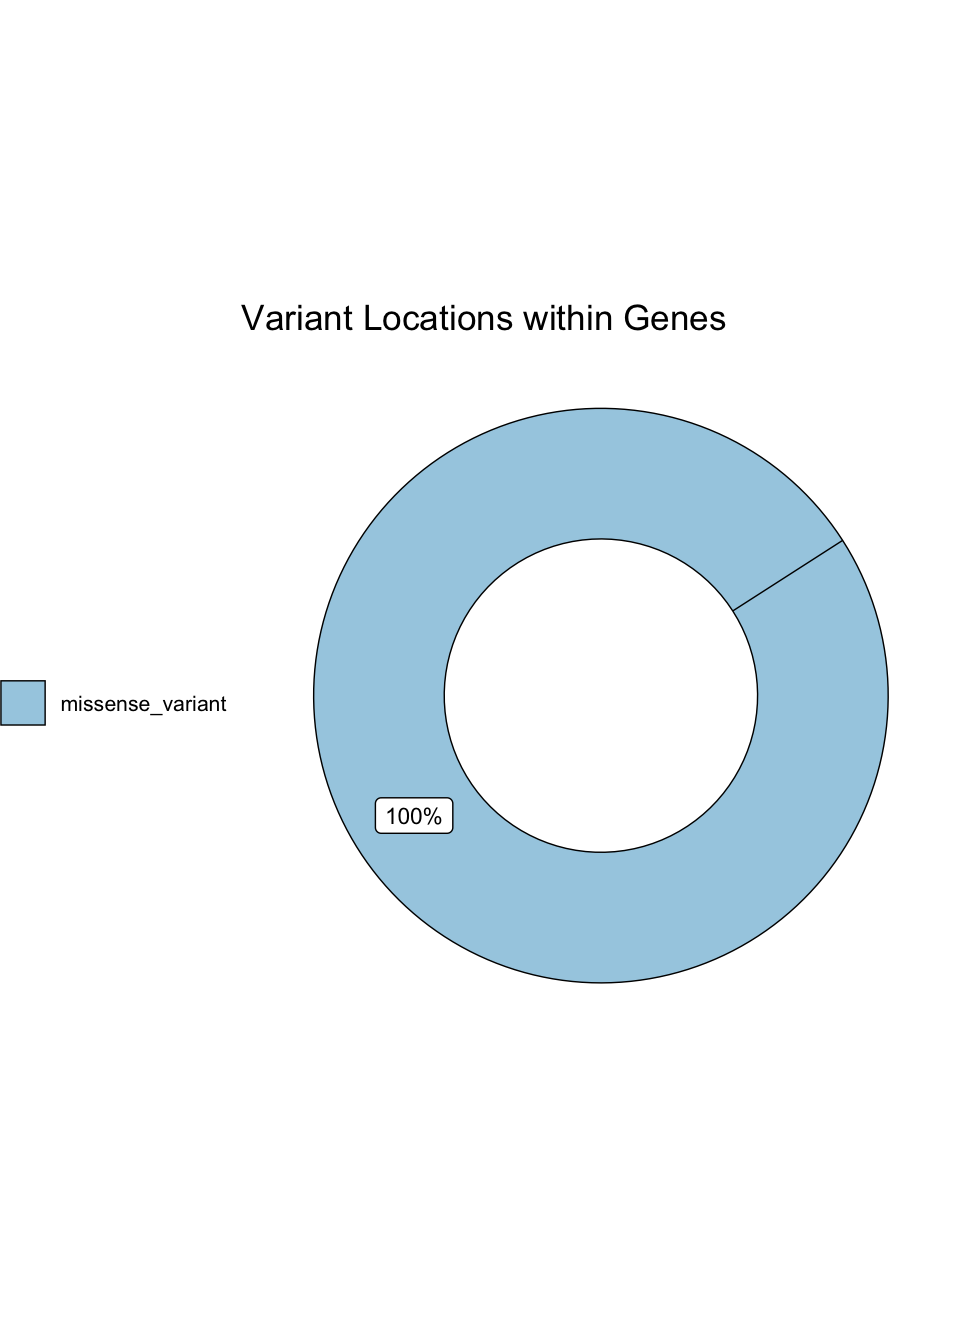
\includegraphics{/Users/jlsmith3/expressed-variant-reporting/reports/Report_HTML_v2_JSmith_files/figure-latex/unnamed-chunk-20-1} 

}

\caption{Figure 1. Percentage of different types of mutations identified.}\label{fig:unnamed-chunk-20}
\end{figure}

\begin{center}\rule{0.5\linewidth}{0.5pt}\end{center}

\begin{center}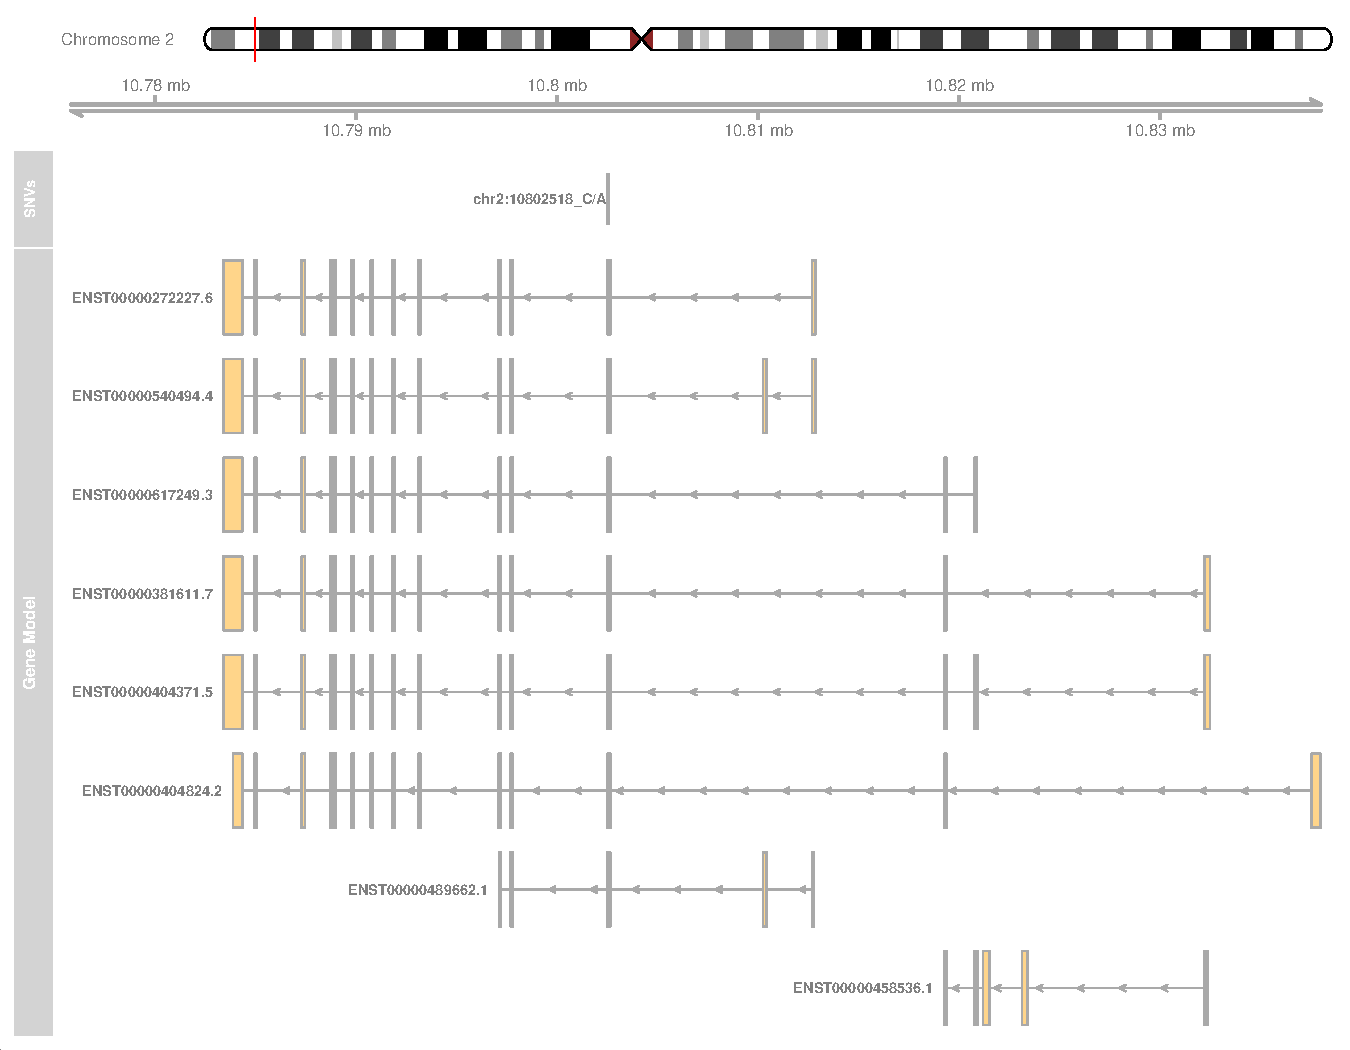
\includegraphics{/Users/jlsmith3/expressed-variant-reporting/reports/Report_HTML_v2_JSmith_files/figure-latex/unnamed-chunk-22-1} 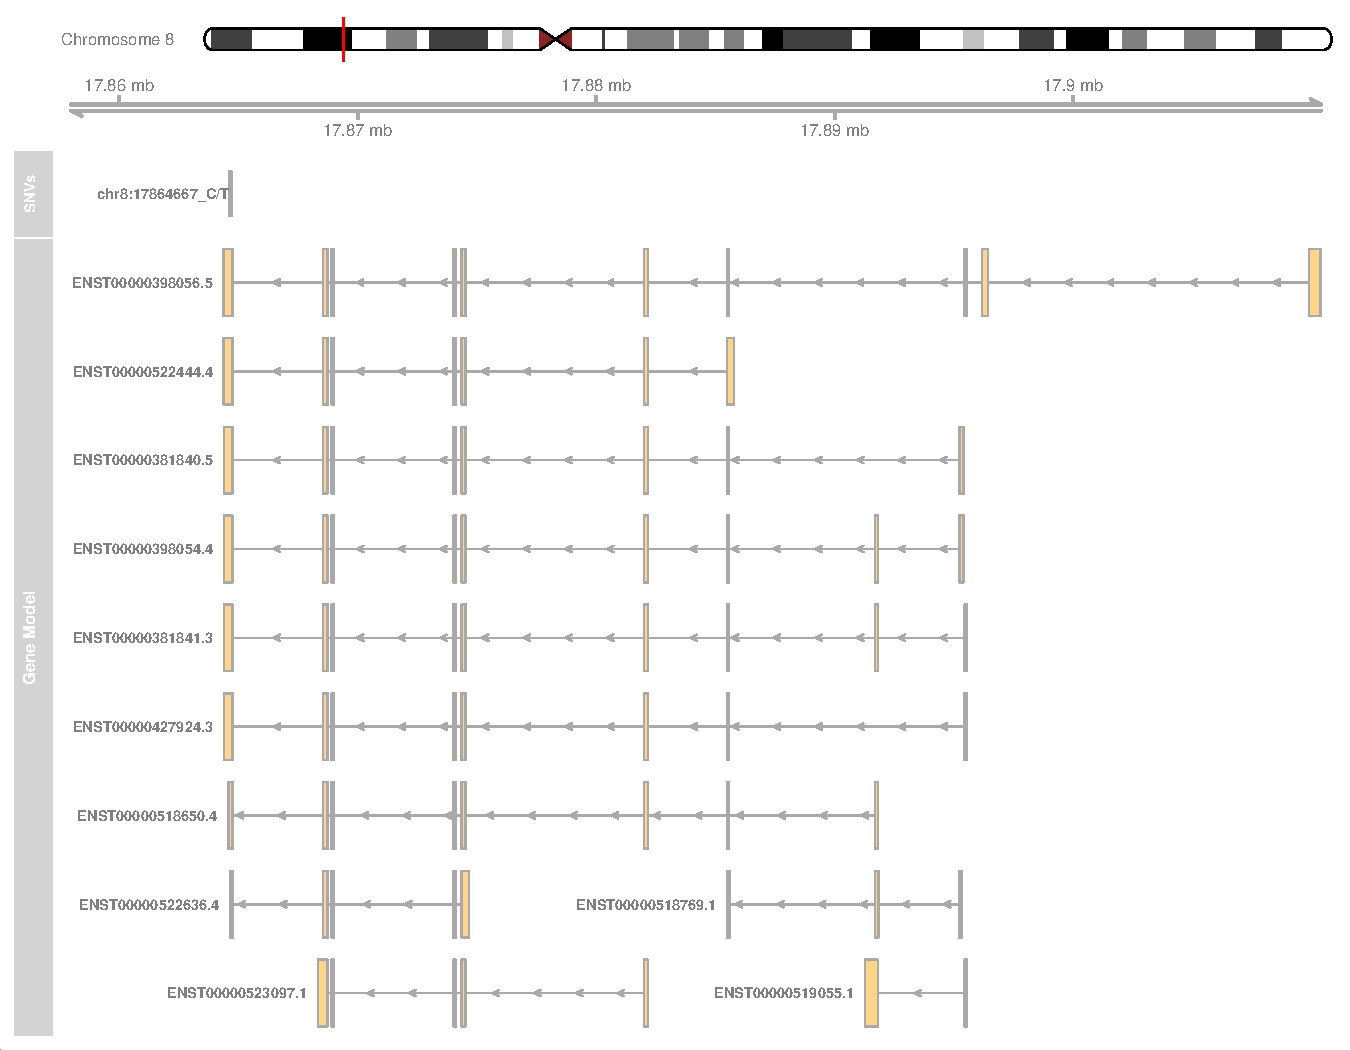
\includegraphics{/Users/jlsmith3/expressed-variant-reporting/reports/Report_HTML_v2_JSmith_files/figure-latex/unnamed-chunk-22-2} 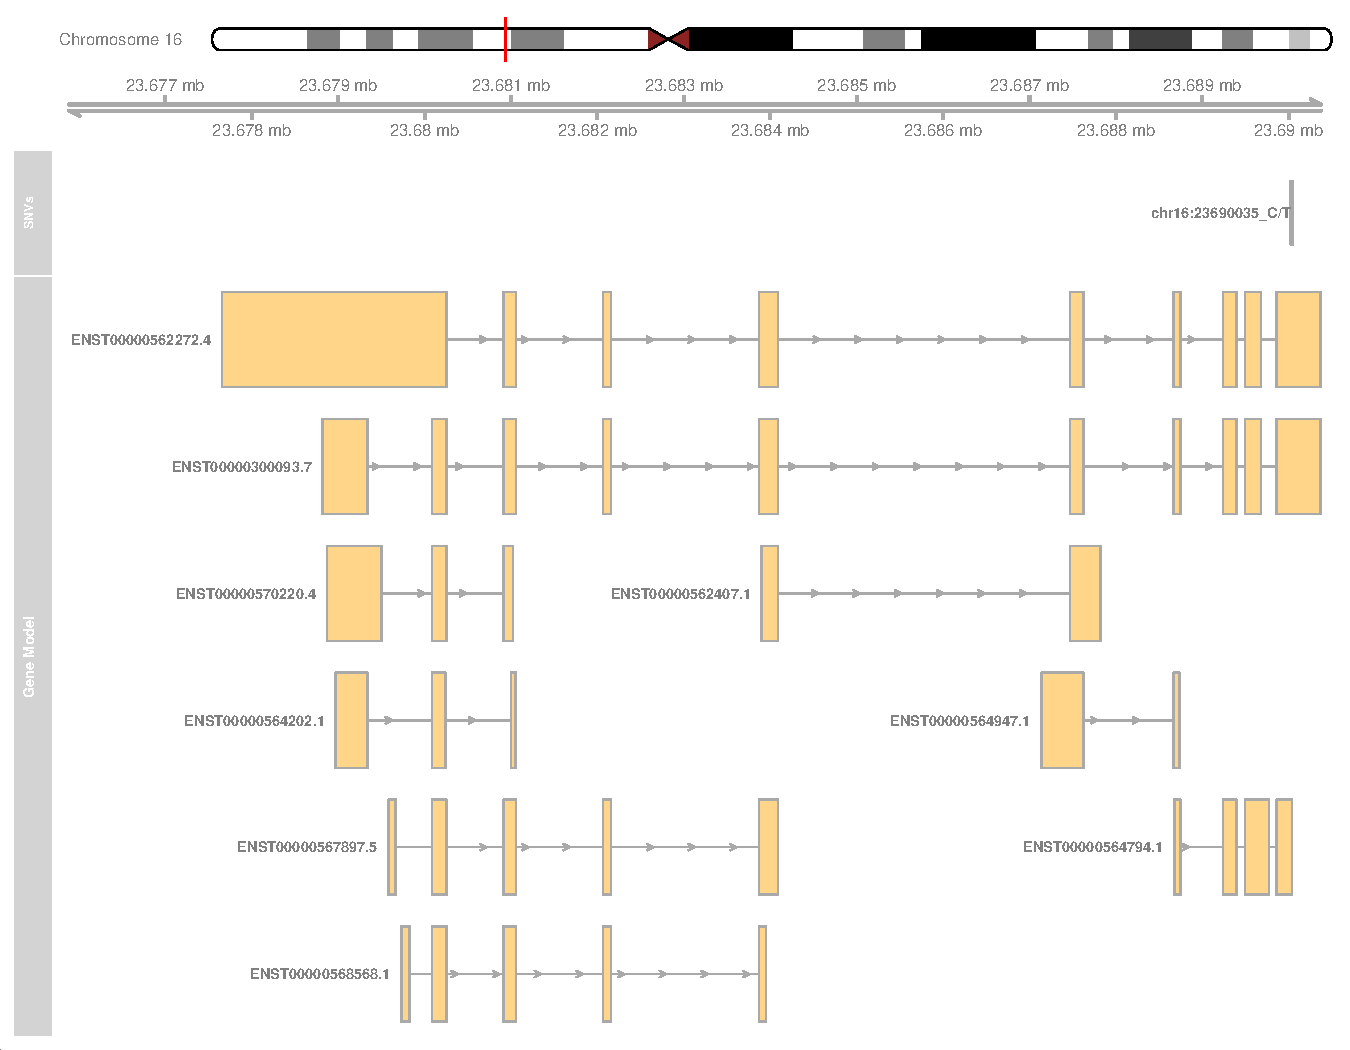
\includegraphics{/Users/jlsmith3/expressed-variant-reporting/reports/Report_HTML_v2_JSmith_files/figure-latex/unnamed-chunk-22-3} \end{center}

\begin{center}\rule{0.5\linewidth}{0.5pt}\end{center}

\begin{Shaded}
\begin{Highlighting}[]
\CommentTok{\# Add Lollipop plot {-} interactive}
\end{Highlighting}
\end{Shaded}

\hypertarget{expression-of-genes-with-mutations}{%
\section{Expression of Genes with
Mutations}\label{expression-of-genes-with-mutations}}

\hypertarget{boxplotsviolin-plots}{%
\section{boxplots/violin plots}\label{boxplotsviolin-plots}}

\begin{verbatim}
##   GeneID.HISAT2.on.data.32..aligned.reads..BAM..HISAT2.on.data.33..aligned.reads..BAM..HISAT2.on.data.34..aligned.reads..BAM..HISAT2.on.data.29..aligned.reads..BAM..HISAT2.on.data.30..aligned.reads..BAM..HISAT2.on.data.31..aligned.reads..BAM.
## 1                                                                                                                      100287102\t0.770218796434557\t0.770218796434554\t0.770218796434557\t0.770218796434557\t0.770218796434557\t0.770218796434557
## 2                                                                                                                         653635\t0.770218796434557\t0.770218796434554\t0.770218796434557\t0.770218796434557\t0.770218796434557\t0.770218796434557
## 3                                                                                                                      102466751\t0.770218796434557\t0.770218796434554\t0.770218796434557\t0.770218796434557\t0.770218796434557\t0.770218796434557
## 4                                                                                                                      100302278\t0.770218796434557\t0.770218796434554\t0.770218796434557\t0.770218796434557\t0.770218796434557\t0.770218796434557
## 5                                                                                                                         645520\t0.770218796434557\t0.770218796434554\t0.770218796434557\t0.770218796434557\t0.770218796434557\t0.770218796434557
## 6                                                                                                                          79501\t0.770218796434557\t0.770218796434554\t0.770218796434557\t0.770218796434557\t0.770218796434557\t0.770218796434557
\end{verbatim}

\hypertarget{de-genes-by-condition}{%
\section{DE genes by condition}\label{de-genes-by-condition}}

\begin{verbatim}
##    GeneID     logFC   logCPM         F      PValue FDR
## 1    5337  7.730171 3.670278 12.958127 0.001712615   1
## 4  146434  7.346030 3.341787 10.349140 0.003722217   1
## 26   3371  6.784363 2.893012  7.379495 0.012078647   1
## 25  80071  6.763869 2.873826  7.379730 0.012077449   1
## 50   4851  6.749349 2.871517  6.598439 0.017991895   1
## 24   1803 -6.887862 3.035071  7.449322 0.011728187   1
\end{verbatim}

\hypertarget{sommelier-results-haplyotypepca}{%
\section{Sommelier results:
Haplyotype/PCA}\label{sommelier-results-haplyotypepca}}

\begin{Shaded}
\begin{Highlighting}[]
\CommentTok{\# add results here}
\end{Highlighting}
\end{Shaded}

\begin{center}\rule{0.5\linewidth}{0.5pt}\end{center}

\hypertarget{what-does-this-result-mean-for-you-and-whats-next}{%
\section{What Does This Result Mean for you? And What's
Next?}\label{what-does-this-result-mean-for-you-and-whats-next}}

Genetic tests sometimes reveal information that could be relevant to
your family such as a health risk that might run in the family, or that
family relationships are different from what you expected.

Can you please add this message in the next steps section, if the report
show an association with a gene. Please contact your doctor and a
genetic counselor. A genetic counselor can help you understand:

\begin{enumerate}
\def\labelenumi{\arabic{enumi}.}
\tightlist
\item
  how your family members may be affected if the test shows a serious
  health condition runs in your family.
\item
  the risk of you and your partner passing on a health condition to your
  children your options if you have a child with an inherited health
  condition and you do not want your next child to inherit it
\item
  genetic counsellor can also direct you to relevant patient support
  group
\end{enumerate}

\begin{Shaded}
\begin{Highlighting}[]
\CommentTok{\# Need diagram here}
\end{Highlighting}
\end{Shaded}

\begin{center}\rule{0.5\linewidth}{0.5pt}\end{center}

\hypertarget{more-information}{%
\section{More information}\label{more-information}}

\hypertarget{recent-publications}{%
\subsection{Recent Publications}\label{recent-publications}}

Quitting from lines 517-529 (Report\_v2\_JSmith.Rmd) Error: Problem with
\texttt{mutate()} input \texttt{GENE}. ✖ Input \texttt{GENE} can't be
recycled to size 20. ℹ Input \texttt{GENE} is
\texttt{rep(genes,\ each\ =\ 5)}. ℹ Input \texttt{GENE} must be size 20
or 1, not 25.

\begin{center}\includegraphics{/Users/jlsmith3/expressed-variant-reporting/reports/Report_HTML_v2_JSmith_files/figure-latex/unnamed-chunk-31-1} \end{center}

\hypertarget{potential-drug-targets}{%
\subsection{Potential Drug Targets}\label{potential-drug-targets}}

Can search for additional drugs that may target the mutant genes online
using \href{http://drugtargetor.com/}{Drug Targetor} and at
\href{https://www.dgidb.org/}{Drug Gene Interaction Database}

\begin{Shaded}
\begin{Highlighting}[]
\CommentTok{\# add drug target data information}
\end{Highlighting}
\end{Shaded}

\hypertarget{potential-clinical-trials}{%
\subsection{Potential Clinical Trials}\label{potential-clinical-trials}}

\begin{Shaded}
\begin{Highlighting}[]
\CommentTok{\# search API at https://clinicaltrials.gov/api/}
\end{Highlighting}
\end{Shaded}

\hypertarget{web-resources}{%
\subsection{Web resources}\label{web-resources}}

\begin{Shaded}
\begin{Highlighting}[]
\CommentTok{\# Add QR code where does it go?}
\end{Highlighting}
\end{Shaded}

\begin{center}\rule{0.5\linewidth}{0.5pt}\end{center}

\hypertarget{consent-for-analysis}{%
\section{Consent for Analysis}\label{consent-for-analysis}}

This should simply be a copy of the consent form the patient has already
signed. Also, interactive shiny widgets make this less portable.

\begin{Shaded}
\begin{Highlighting}[]
\CommentTok{\# Need to have runtime: shiny in the YAML header}
\CommentTok{\# but this makes the Rmd essentially a shiny server}
\CommentTok{\# which limits portability AFAIK}
\CommentTok{\# patient\_signature()}
\end{Highlighting}
\end{Shaded}

\begin{center}\rule{0.5\linewidth}{0.5pt}\end{center}

\hypertarget{quality-control}{%
\section{Quality Control}\label{quality-control}}

\hypertarget{embed-the-igv-output-from-ctat-mutation-pipeline.}{%
\subsection{Embed the IGV output from CTAT Mutation
pipeline.}\label{embed-the-igv-output-from-ctat-mutation-pipeline.}}

\begin{Shaded}
\begin{Highlighting}[]
\CommentTok{\# embed file here}
\end{Highlighting}
\end{Shaded}

\hypertarget{sequencing-depth-and-qc}{%
\subsection{Sequencing Depth and QC}\label{sequencing-depth-and-qc}}

\begin{Shaded}
\begin{Highlighting}[]
\CommentTok{\# include Deeptools plots for coverage, average}
\CommentTok{\# base quality scores, alignment quality scores,}
\CommentTok{\# etc.}
\end{Highlighting}
\end{Shaded}

\begin{center}\rule{0.5\linewidth}{0.5pt}\end{center}

\hypertarget{references}{%
\section{References:}\label{references}}

\hypertarget{citations}{%
\subsection{Citations}\label{citations}}

\emph{Smith RN, et al.~InterMine: a flexible data warehouse system for
the integration and analysis of heterogeneous biological data.
Bioinformatics. 2012 Dec 1;28(23):3163-5.}

\hypertarget{genome-references-and-software}{%
\subsection{Genome References and
Software}\label{genome-references-and-software}}

\hypertarget{additional-information-about-the-pipelines-used-check-out-the-github-repositories-listed-below}{%
\subsection{Additional information about the pipelines used, check out
the github repositories listed
below:}\label{additional-information-about-the-pipelines-used-check-out-the-github-repositories-listed-below}}

\begin{itemize}
\tightlist
\item
  \href{https://github.com/collaborativebioinformatics/expressed-variant-impact}{CTAT
  Mutation Pipeline for Input VCF}
\item
  \href{https://github.com/collaborativebioinformatics/viravate2}{Association
  between Genes and Drug Targets}
\item
  \href{https://github.com/collaborativebioinformatics/mixed-sample-graphs}{Mixed
  Sample Graphs QC}
\item
  \href{https://github.com/collaborativebioinformatics/expressed-variant-reporting}{snpReportR
  Generation}
\item
  \href{https://chasmplus.readthedocs.io/en/latest/index.html}{CHASMplus}
\item
  \href{http://fathmm.biocompute.org.uk/}{FATHMM}
\item
  \href{https://karchinlab.org/apps/appVest.html}{VEST}
\end{itemize}

\begin{center}\includegraphics{/Users/jlsmith3/expressed-variant-reporting/reports/Report_HTML_v2_JSmith_files/figure-latex/unnamed-chunk-39-1} \end{center}

\begin{verbatim}
## TxDb object:
## # Db type: TxDb
## # Supporting package: GenomicFeatures
## # Data source: ~/Downloads/gencode.v22.annotation.gtf.gz
## # Organism: NA
## # Taxonomy ID: NA
## # miRBase build ID: NA
## # Genome: NA
## # Nb of transcripts: 198442
## # Db created by: GenomicFeatures package from Bioconductor
## # Creation time: 2021-03-30 19:49:41 -0700 (Tue, 30 Mar 2021)
## # GenomicFeatures version at creation time: 1.42.2
## # RSQLite version at creation time: 2.2.5
## # DBSCHEMAVERSION: 1.2
\end{verbatim}

\hypertarget{session-information}{%
\subsection{Session Information}\label{session-information}}

\begin{Shaded}
\begin{Highlighting}[]
\FunctionTok{sessionInfo}\NormalTok{()}
\end{Highlighting}
\end{Shaded}

\begin{verbatim}
## R version 4.0.4 (2021-02-15)
## Platform: x86_64-apple-darwin17.0 (64-bit)
## Running under: macOS Catalina 10.15.7
## 
## Matrix products: default
## BLAS:   /Library/Frameworks/R.framework/Versions/4.0/Resources/lib/libRblas.dylib
## LAPACK: /Library/Frameworks/R.framework/Versions/4.0/Resources/lib/libRlapack.dylib
## 
## locale:
## [1] C/en_US.UTF-8/en_US.UTF-8/C/en_US.UTF-8/en_US.UTF-8
## 
## attached base packages:
##  [1] grid      stats4    parallel  stats     graphics  grDevices utils    
##  [8] datasets  methods   base     
## 
## other attached packages:
##  [1] Gviz_1.34.1                 VariantAnnotation_1.36.0   
##  [3] Rsamtools_2.6.0             Biostrings_2.58.0          
##  [5] XVector_0.30.0              SummarizedExperiment_1.20.0
##  [7] MatrixGenerics_1.2.1        matrixStats_0.58.0         
##  [9] vcfR_1.12.0                 RColorBrewer_1.1-2         
## [11] gridExtra_2.3               ggplot2_3.3.3              
## [13] shiny_1.6.0                 stringr_1.4.0              
## [15] magrittr_2.0.1              knitr_1.31                 
## [17] GenomicFeatures_1.42.2      AnnotationDbi_1.52.0       
## [19] Biobase_2.50.0              GenomicRanges_1.42.0       
## [21] GenomeInfoDb_1.26.4         IRanges_2.24.1             
## [23] S4Vectors_0.28.1            BiocGenerics_0.36.0        
## [25] here_1.0.1                  rmarkdown_2.7              
## [27] tidyr_1.1.3                 dplyr_1.0.5                
## [29] jsonlite_1.7.2              InterMineR_1.12.0          
## 
## loaded via a namespace (and not attached):
##   [1] utf8_1.2.1               proto_1.0.0              tidyselect_1.1.0        
##   [4] RSQLite_2.2.5            htmlwidgets_1.5.3        BiocParallel_1.24.1     
##   [7] devtools_2.3.2           munsell_0.5.0            chron_2.3-56            
##  [10] DT_0.17                  withr_2.4.1              colorspace_2.0-0        
##  [13] highr_0.8                rstudioapi_0.13          labeling_0.4.2          
##  [16] GenomeInfoDbData_1.2.4   farver_2.1.0             bit64_4.0.5             
##  [19] rprojroot_2.0.2          vctrs_0.3.6              generics_0.1.0          
##  [22] xfun_0.22                biovizBase_1.38.0        BiocFileCache_1.14.0    
##  [25] R6_2.5.0                 RJSONIO_1.3-1.4          AnnotationFilter_1.14.0 
##  [28] bitops_1.0-6             cachem_1.0.4             DelayedArray_0.16.3     
##  [31] assertthat_0.2.1         promises_1.2.0.1         scales_1.1.1            
##  [34] pinfsc50_1.2.0           nnet_7.3-15              debugme_1.1.0           
##  [37] gtable_0.3.0             processx_3.5.0           ensembldb_2.14.0        
##  [40] rlang_0.4.10             systemfonts_1.0.1        splines_4.0.4           
##  [43] rtracklayer_1.50.0       lazyeval_0.2.2           gargle_1.0.0            
##  [46] dichromat_2.0-0          checkmate_2.0.0          yaml_2.2.1              
##  [49] crosstalk_1.1.1          backports_1.2.1          httpuv_1.5.5            
##  [52] Hmisc_4.5-0              tools_4.0.4              usethis_2.0.1           
##  [55] ellipsis_0.3.1           kableExtra_1.3.4         jquerylib_0.1.3         
##  [58] sessioninfo_1.1.1        gsubfn_0.7               Rcpp_1.0.6              
##  [61] base64enc_0.1-3          progress_1.2.2           zlibbioc_1.36.0         
##  [64] purrr_0.3.4              RCurl_1.98-1.3           ps_1.6.0                
##  [67] prettyunits_1.1.1        rpart_4.1-15             openssl_1.4.3           
##  [70] sqldf_0.4-11             ggrepel_0.9.1            cluster_2.1.1           
##  [73] fs_1.5.0                 data.table_1.14.0        snpReportR_0.0.0.9      
##  [76] ProtGenerics_1.22.0      pkgload_1.2.0            hms_1.0.0               
##  [79] mime_0.10                evaluate_0.14            xtable_1.8-4            
##  [82] XML_3.99-0.6             jpeg_0.1-8.1             gmailr_1.0.0            
##  [85] testthat_3.0.2           compiler_4.0.4           biomaRt_2.46.3          
##  [88] tibble_3.1.0             crayon_1.4.1             htmltools_0.5.1.1       
##  [91] mgcv_1.8-34              later_1.1.0.1            Formula_1.2-4           
##  [94] DBI_1.1.1                formatR_1.8              dbplyr_2.1.0            
##  [97] MASS_7.3-53.1            rappdirs_0.3.3           Matrix_1.3-2            
## [100] permute_0.9-5            cli_2.3.1                igraph_1.2.6            
## [103] pkgconfig_2.0.3          GenomicAlignments_1.26.0 foreign_0.8-81          
## [106] xml2_1.3.2               roxygen2_7.1.1           memuse_4.1-0            
## [109] svglite_2.0.0            bslib_0.2.4              webshot_0.5.2           
## [112] rvest_1.0.0              callr_3.6.0              digest_0.6.27           
## [115] vegan_2.5-7              htmlTable_2.1.0          curl_4.3                
## [118] lifecycle_1.0.0          nlme_3.1-152             desc_1.3.0              
## [121] viridisLite_0.3.0        askpass_1.1              BSgenome_1.58.0         
## [124] fansi_0.4.2              pillar_1.5.1             lattice_0.20-41         
## [127] fastmap_1.1.0            httr_1.4.2               pkgbuild_1.2.0          
## [130] survival_3.2-10          glue_1.4.2               remotes_2.2.0           
## [133] png_0.1-7                bit_4.0.4                stringi_1.5.3           
## [136] sass_0.3.1               blob_1.2.1               latticeExtra_0.6-29     
## [139] memoise_2.0.0            ape_5.4-1
\end{verbatim}

\end{document}
